\documentclass[tikz,margin=0cm,dvipsnames,x11names,rgb]{standalone}

\usepackage{amsmath,amssymb,amsfonts}
\usetikzlibrary{calc,
fit,
shapes.misc,
shapes.geometric,
arrows.meta,
fadings,
matrix,
chains,
scopes,
positioning}

\usepackage{pgfplots}
\usepackage{pgfplotstable}
\pgfplotsset{compat=1.18}



\usepackage[]{fontspec}

\setmainfont{Latin Modern Roman}
\setmonofont{Latin Modern Math}
\renewcommand{\textsc}[1]{{\fontfamily{lmr}\selectfont \scshape #1}}

\usepackage[]{bm}

\makeatletter
\@ifundefined{fromRoot}{\newcommand{\fromRoot}[1]{../../#1}}{}

\def\input@path{{../..}{..}{.}{./svg}{./pgfplots}{./tikzpicture}}
%or: \def\input@path{{/path/to/folder/}{/path/to/other/folder/}}
\makeatother

\newcommand{\ra}[1]{\renewcommand{\arraystretch}{#1}}

\newcommand*{\gf}[1]{\acrshort{gf}($#1$)}%
\newcommand*{\mpn}[1]{\bm{P}_{#1}}%
\newcommand*{\pn}[1]{%
  \ifthenelse{\equal{#1}{}}{$\mpn{0}$}{$\mpn{#1}$}%
}%

\newcommand*{\pk}[3]{%
  \ifthenelse{\equal{#1}{#2}}{\textcolor{red}{\phantom{.}$p_0$\phantom{.}}}{\phantom{.}$p_#3$\phantom{.}}%
}%


\newcommand*{\placeholderreg}{\includegraphics[width=\linewidth, height=.25\textheight, keepaspectratio = true]{figures/certified_xilinx.png}}%
\newcommand*{\placeholder}[1]{\includegraphics[#1]{figures/certified_xilinx.png}}%

\newcommand*{\snr}{\acrshort{snr}}%
\newcommand*{\snrs}{\acrshortpl{snr}}%

\newcommand*{\mpd}[0]{p_\Delta}%
\newcommand*{\mpo}[0]{p_\omega}%
\newcommand*{\pd}[0]{$\mpd$}%
\newcommand*{\po}[0]{$\mpo$}%
\newcommand*{\mpfa}[0]{\mathcal{P}_{fa}}%
\newcommand*{\mpmd}[0]{\mathcal{P}_{md}}%
\newcommand*{\pfa}[0]{\acrshort{pfa}}%
\newcommand*{\pmd}[0]{\acrshort{pmd}}%
\newcommand*{\mnorm}[1]{\mathcal{L}_{#1}}%
\newcommand*{\norm}[1]{$\mnorm{#1}$}%
\newcommand*{\fft}{\acrshort{fft}}%
\newcommand*{\mfft}[1]{\mathcal{F}(#1)}%
\newcommand*{\mifft}[1]{\mathcal{F}^{-1}(#1)}%
\newcommand*{\ts}{\acrshort{ts}}%

\newcommand*{\cpp}[1]{C\textrm{++#1}}%
\newcommand*{\na}{\textrm{\textcolor{SlateGray4}{N/A}}}%

\newcommand*{\vect}[1]{\bm{#1}}%
\newcommand*{\mat}[1]{\bm{\mathrm{#1}}}%

\newcommand*{\task}[1]{\mathcal{T}_{#1}}%

\newcommand*{\sdr}{\acrshort{sdr}}%
\newcommand*{\fpga}{\acrshort{fpga}}%

\newcommand*{\rikiki}{\fontsize{4}{6}\selectfont}%


\pgfdeclarelayer{background}
\pgfsetlayers{background, main}

\begin{document}

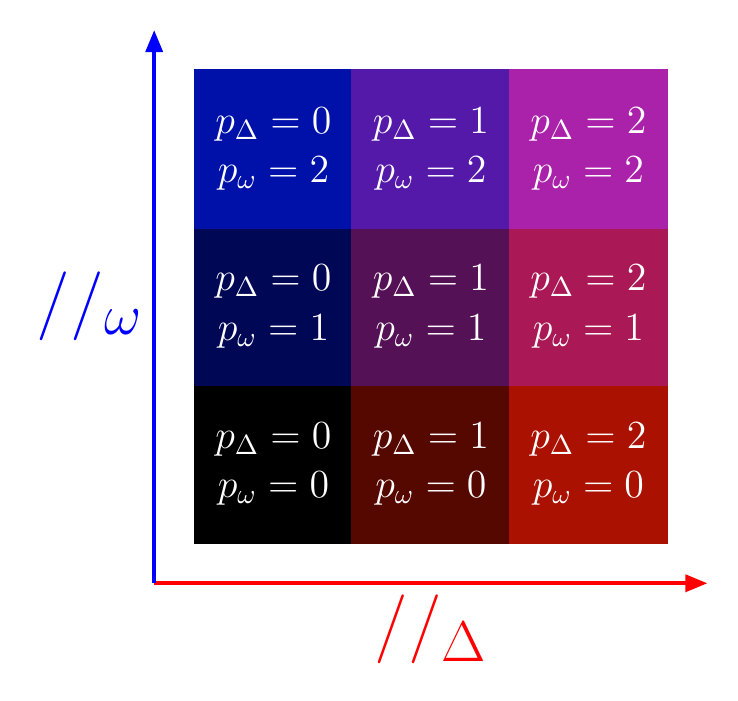
\begin{tikzpicture} [->,
  >={Triangle[width=6pt, length=8pt]},
  auto,
  thick,
  font={\Large}]

  \def\expf{2}
  \def\vpw{3}
  \def\vpd{3}

  \foreach \n [
    evaluate = \n as \nm using int(\n - 1),
    evaluate = \n as \rcolor using (\nm * 1 / \vpd),
    evaluate = \n as \x using (\n * \expf),
  ] in {1,...,\vpd}
    {
      \foreach \w [
          evaluate = \w as \wm using int(\w - 1),
        evaluate = \w as \bcolor using (\wm * 1 / \vpw),
        evaluate = \w as \y using (\w * \expf),
        evaluate = \w as \gcolor using ((\bcolor + \rcolor) * .1),
      ] in {1,...,\vpw}
        {
          \definecolor{clr\n\w}{rgb}{\rcolor, \gcolor, \bcolor}

          \node [
            clr\n\w,
            fill,
            draw,
            minimum size = \expf cm,
            align = center,
            text = white,
          ] (n\n\w) at (\x, \y) {$\mpd{} = \nm$\\$\mpo{} = \wm$};
        }
    }

  \draw [ultra thick, Red,]
  ($(n11.south west) + (-.5, -.5)$) -- ($(n\vpw1.south east) + (.5, -.5)$)
  node [font={\Huge}, midway, below, Red] {$//_{\Delta}$};
  \draw [ultra thick, Blue,]
  ($(n11.south west) + (-.5, -.5)$) -- ($(n1\vpd.north west) + (-.5, .5)$)
  node [font={\Huge}, midway, left, Blue] {$//_{\omega}$};

\end{tikzpicture}
\end{document}
